
%% bare_conf.tex
%% V1.3
%% 2007/01/11
%% by Michael Shell
%% See:
%% http://www.michaelshell.org/
%% for current contact information.
%%
%% This is a skeleton file demonstrating the use of IEEEtran.cls
%% (requires IEEEtran.cls version 1.7 or later) with an IEEE conference paper.
%%
%% Support sites:
%% http://www.michaelshell.org/tex/ieeetran/
%% http://www.ctan.org/tex-archive/macros/latex/contrib/IEEEtran/
%% and
%% http://www.ieee.org/

%%*************************************************************************
%% Legal Notice:
%% This code is offered as-is without any warranty either expressed or
%% implied; without even the implied warranty of MERCHANTABILITY or
%% FITNESS FOR A PARTICULAR PURPOSE! 
%% User assumes all risk.
%% In no event shall IEEE or any contributor to this code be liable for
%% any damages or losses, including, but not limited to, incidental,
%% consequential, or any other damages, resulting from the use or misuse
%% of any information contained here.
%%
%% All comments are the opinions of their respective authors and are not
%% necessarily endorsed by the IEEE.
%%
%% This work is distributed under the LaTeX Project Public License (LPPL)
%% ( http://www.latex-project.org/ ) version 1.3, and may be freely used,
%% distributed and modified. A copy of the LPPL, version 1.3, is included
%% in the base LaTeX documentation of all distributions of LaTeX released
%% 2003/12/01 or later.
%% Retain all contribution notices and credits.
%% ** Modified files should be clearly indicated as such, including  **
%% ** renaming them and changing author support contact information. **
%%
%% File list of work: IEEEtran.cls, IEEEtran_HOWTO.pdf, bare_adv.tex,
%%                    bare_conf.tex, bare_jrnl.tex, bare_jrnl_compsoc.tex
%%*************************************************************************

% *** Authors should verify (and, if needed, correct) their LaTeX system  ***
% *** with the testflow diagnostic prior to trusting their LaTeX platform ***
% *** with production work. IEEE's font choices can trigger bugs that do  ***
% *** not appear when using other class files.                            ***
% The testflow support page is at:
% http://www.michaelshell.org/tex/testflow/



% Note that the a4paper option is mainly intended so that authors in
% countries using A4 can easily print to A4 and see how their papers will
% look in print - the typesetting of the document will not typically be
% affected with changes in paper size (but the bottom and side margins will).
% Use the testflow package mentioned above to verify correct handling of
% both paper sizes by the user's LaTeX system.
%
% Also note that the "draftcls" or "draftclsnofoot", not "draft", option
% should be used if it is desired that the figures are to be displayed in
% draft mode.
%
\documentclass[10pt, conference]{IEEEtran}

\usepackage[para]{footmisc}
\usepackage{url}
\usepackage{verbatim}
\usepackage{graphicx}

% Add the compsocconf option for Computer Society conferences.
%
% If IEEEtran.cls has not been installed into the LaTeX system files,
% manually specify the path to it like:
% \documentclass[conference]{../sty/IEEEtran}


% Some very useful LaTeX packages include:
% (uncomment the ones you want to load)


% *** MISC UTILITY PACKAGES ***
%
%\usepackage{ifpdf}
% Heiko Oberdiek's ifpdf.sty is very useful if you need conditional
% compilation based on whether the output is pdf or dvi.
% usage:
% \ifpdf
%   % pdf code
% \else
%   % dvi code
% \fi
% The latest version of ifpdf.sty can be obtained from:
% http://www.ctan.org/tex-archive/macros/latex/contrib/oberdiek/
% Also, note that IEEEtran.cls V1.7 and later provides a builtin
% \ifCLASSINFOpdf conditional that works the same way.
% When switching from latex to pdflatex and vice-versa, the compiler may
% have to be run twice to clear warning/error messages.






% *** CITATION PACKAGES ***
%
%\usepackage{cite}
% cite.sty was written by Donald Arseneau
% V1.6 and later of IEEEtran pre-defines the format of the cite.sty package
% \cite{} output to follow that of IEEE. Loading the cite package will
% result in citation numbers being automatically sorted and properly
% "compressed/ranged". e.g., [1], [9], [2], [7], [5], [6] without using
% cite.sty will become [1], [2], [5]--[7], [9] using cite.sty. cite.sty's
% \cite will automatically add leading space, if needed. Use cite.sty's
% noadjust option (cite.sty V3.8 and later) if you want to turn this off.
% cite.sty is already installed on most LaTeX systems. Be sure and use
% version 4.0 (2003-05-27) and later if using hyperref.sty. cite.sty does
% not currently provide for hyperlinked citations.
% The latest version can be obtained at:
% http://www.ctan.org/tex-archive/macros/latex/contrib/cite/
% The documentation is contained in the cite.sty file itself.






% *** GRAPHICS RELATED PACKAGES ***
%
\ifCLASSINFOpdf
  % \usepackage[pdftex]{graphicx}
  % declare the path(s) where your graphic files are
  % \graphicspath{{../pdf/}{../jpeg/}}
  % and their extensions so you won't have to specify these with
  % every instance of \includegraphics
  % \DeclareGraphicsExtensions{.pdf,.jpeg,.png}
\else
  % or other class option (dvipsone, dvipdf, if not using dvips). graphicx
  % will default to the driver specified in the system graphics.cfg if no
  % driver is specified.
  % \usepackage[dvips]{graphicx}
  % declare the path(s) where your graphic files are
  % \graphicspath{{../eps/}}
  % and their extensions so you won't have to specify these with
  % every instance of \includegraphics
  % \DeclareGraphicsExtensions{.eps}
\fi
% graphicx was written by David Carlisle and Sebastian Rahtz. It is
% required if you want graphics, photos, etc. graphicx.sty is already
% installed on most LaTeX systems. The latest version and documentation can
% be obtained at: 
% http://www.ctan.org/tex-archive/macros/latex/required/graphics/
% Another good source of documentation is "Using Imported Graphics in
% LaTeX2e" by Keith Reckdahl which can be found as epslatex.ps or
% epslatex.pdf at: http://www.ctan.org/tex-archive/info/
%
% latex, and pdflatex in dvi mode, support graphics in encapsulated
% postscript (.eps) format. pdflatex in pdf mode supports graphics
% in .pdf, .jpeg, .png and .mps (metapost) formats. Users should ensure
% that all non-photo figures use a vector format (.eps, .pdf, .mps) and
% not a bitmapped formats (.jpeg, .png). IEEE frowns on bitmapped formats
% which can result in "jaggedy"/blurry rendering of lines and letters as
% well as large increases in file sizes.
%
% You can find documentation about the pdfTeX application at:
% http://www.tug.org/applications/pdftex





% *** MATH PACKAGES ***
%
%\usepackage[cmex10]{amsmath}
% A popular package from the American Mathematical Society that provides
% many useful and powerful commands for dealing with mathematics. If using
% it, be sure to load this package with the cmex10 option to ensure that
% only type 1 fonts will utilized at all point sizes. Without this option,
% it is possible that some math symbols, particularly those within
% footnotes, will be rendered in bitmap form which will result in a
% document that can not be IEEE Xplore compliant!
%
% Also, note that the amsmath package sets \interdisplaylinepenalty to 10000
% thus preventing page breaks from occurring within multiline equations. Use:
%\interdisplaylinepenalty=2500
% after loading amsmath to restore such page breaks as IEEEtran.cls normally
% does. amsmath.sty is already installed on most LaTeX systems. The latest
% version and documentation can be obtained at:
% http://www.ctan.org/tex-archive/macros/latex/required/amslatex/math/





% *** SPECIALIZED LIST PACKAGES ***
%
%\usepackage{algorithmic}
% algorithmic.sty was written by Peter Williams and Rogerio Brito.
% This package provides an algorithmic environment fo describing algorithms.
% You can use the algorithmic environment in-text or within a figure
% environment to provide for a floating algorithm. Do NOT use the algorithm
% floating environment provided by algorithm.sty (by the same authors) or
% algorithm2e.sty (by Christophe Fiorio) as IEEE does not use dedicated
% algorithm float types and packages that provide these will not provide
% correct IEEE style captions. The latest version and documentation of
% algorithmic.sty can be obtained at:
% http://www.ctan.org/tex-archive/macros/latex/contrib/algorithms/
% There is also a support site at:
% http://algorithms.berlios.de/index.html
% Also of interest may be the (relatively newer and more customizable)
% algorithmicx.sty package by Szasz Janos:
% http://www.ctan.org/tex-archive/macros/latex/contrib/algorithmicx/




% *** ALIGNMENT PACKAGES ***
%
%\usepackage{array}
% Frank Mittelbach's and David Carlisle's array.sty patches and improves
% the standard LaTeX2e array and tabular environments to provide better
% appearance and additional user controls. As the default LaTeX2e table
% generation code is lacking to the point of almost being broken with
% respect to the quality of the end results, all users are strongly
% advised to use an enhanced (at the very least that provided by array.sty)
% set of table tools. array.sty is already installed on most systems. The
% latest version and documentation can be obtained at:
% http://www.ctan.org/tex-archive/macros/latex/required/tools/


%\usepackage{mdwmath}
%\usepackage{mdwtab}
% Also highly recommended is Mark Wooding's extremely powerful MDW tools,
% especially mdwmath.sty and mdwtab.sty which are used to format equations
% and tables, respectively. The MDWtools set is already installed on most
% LaTeX systems. The lastest version and documentation is available at:
% http://www.ctan.org/tex-archive/macros/latex/contrib/mdwtools/


% IEEEtran contains the IEEEeqnarray family of commands that can be used to
% generate multiline equations as well as matrices, tables, etc., of high
% quality.


%\usepackage{eqparbox}
% Also of notable interest is Scott Pakin's eqparbox package for creating
% (automatically sized) equal width boxes - aka "natural width parboxes".
% Available at:
% http://www.ctan.org/tex-archive/macros/latex/contrib/eqparbox/





% *** SUBFIGURE PACKAGES ***
%\usepackage[tight,footnotesize]{subfigure}
% subfigure.sty was written by Steven Douglas Cochran. This package makes it
% easy to put subfigures in your figures. e.g., "Figure 1a and 1b". For IEEE
% work, it is a good idea to load it with the tight package option to reduce
% the amount of white space around the subfigures. subfigure.sty is already
% installed on most LaTeX systems. The latest version and documentation can
% be obtained at:
% http://www.ctan.org/tex-archive/obsolete/macros/latex/contrib/subfigure/
% subfigure.sty has been superceeded by subfig.sty.



%\usepackage[caption=false]{caption}
%\usepackage[font=footnotesize]{subfig}
% subfig.sty, also written by Steven Douglas Cochran, is the modern
% replacement for subfigure.sty. However, subfig.sty requires and
% automatically loads Axel Sommerfeldt's caption.sty which will override
% IEEEtran.cls handling of captions and this will result in nonIEEE style
% figure/table captions. To prevent this problem, be sure and preload
% caption.sty with its "caption=false" package option. This is will preserve
% IEEEtran.cls handing of captions. Version 1.3 (2005/06/28) and later 
% (recommended due to many improvements over 1.2) of subfig.sty supports
% the caption=false option directly:
%\usepackage[caption=false,font=footnotesize]{subfig}
%
% The latest version and documentation can be obtained at:
% http://www.ctan.org/tex-archive/macros/latex/contrib/subfig/
% The latest version and documentation of caption.sty can be obtained at:
% http://www.ctan.org/tex-archive/macros/latex/contrib/caption/




% *** FLOAT PACKAGES ***
%
%\usepackage{fixltx2e}
% fixltx2e, the successor to the earlier fix2col.sty, was written by
% Frank Mittelbach and David Carlisle. This package corrects a few problems
% in the LaTeX2e kernel, the most notable of which is that in current
% LaTeX2e releases, the ordering of single and double column floats is not
% guaranteed to be preserved. Thus, an unpatched LaTeX2e can allow a
% single column figure to be placed prior to an earlier double column
% figure. The latest version and documentation can be found at:
% http://www.ctan.org/tex-archive/macros/latex/base/



%\usepackage{stfloats}
% stfloats.sty was written by Sigitas Tolusis. This package gives LaTeX2e
% the ability to do double column floats at the bottom of the page as well
% as the top. (e.g., "\begin{figure*}[!b]" is not normally possible in
% LaTeX2e). It also provides a command:
%\fnbelowfloat
% to enable the placement of footnotes below bottom floats (the standard
% LaTeX2e kernel puts them above bottom floats). This is an invasive package
% which rewrites many portions of the LaTeX2e float routines. It may not work
% with other packages that modify the LaTeX2e float routines. The latest
% version and documentation can be obtained at:
% http://www.ctan.org/tex-archive/macros/latex/contrib/sttools/
% Documentation is contained in the stfloats.sty comments as well as in the
% presfull.pdf file. Do not use the stfloats baselinefloat ability as IEEE
% does not allow \baselineskip to stretch. Authors submitting work to the
% IEEE should note that IEEE rarely uses double column equations and
% that authors should try to avoid such use. Do not be tempted to use the
% cuted.sty or midfloat.sty packages (also by Sigitas Tolusis) as IEEE does
% not format its papers in such ways.





% *** PDF, URL AND HYPERLINK PACKAGES ***
%
%\usepackage{url}
% url.sty was written by Donald Arseneau. It provides better support for
% handling and breaking URLs. url.sty is already installed on most LaTeX
% systems. The latest version can be obtained at:
% http://www.ctan.org/tex-archive/macros/latex/contrib/misc/
% Read the url.sty source comments for usage information. Basically,
% \url{my_url_here}.

% *** Do not adjust lengths that control margins, column widths, etc. ***
% *** Do not use packages that alter fonts (such as pslatex).         ***
% There should be no need to do such things with IEEEtran.cls V1.6 and later.
% (Unless specifically asked to do so by the journal or conference you plan
% to submit to, of course. )

% correct bad hyphenation here
\hyphenation{op-tical net-works semi-conduc-tor}

\begin{document}
%
% paper title
% can use linebreaks \\ within to get better formatting as desired
\title{Social Coding with Code Reviews inside the IDE}


% author names and affiliations
% use a multiple column layout for up to two cterent
% affiliations

\author{\IEEEauthorblockN{Tobias D{\"u}rschmid}
\IEEEauthorblockA{%Computer Graphics\\
Hasso Plattner Institute, University of Potsdam, Germany\\
tobias.duerschmid@student.hpi.de}
}

% conference papers do not typically use \thanks and this command
% is locked out in conference mode. If really needed, such as for
% the acknowledgment of grants, issue a \IEEEoverridecommandlockouts
% after \documentclass

% for over three affiliations, or if they all won't fit within the width
% of the page, use this alternative format:
% 
%\author{\IEEEauthorblockN{Michael Shell\IEEEauthorrefmark{1},
%Homer Simpson\IEEEauthorrefmark{2},
%James Kirk\IEEEauthorrefmark{3}, 
%Montgomery Scott\IEEEauthorrefmark{3} and
%Eldon Tyrell\IEEEauthorrefmark{4}}
%\IEEEauthorblockA{\IEEEauthorrefmark{1}School of Electrical and Computer Engineering\\
%Georgia Institute of Technology,
%Atlanta, Georgia 30332--0250\\ Email: see http://www.michaelshell.org/contact.html}
%\IEEEauthorblockA{\IEEEauthorrefmark{2}Twentieth Century Fox, Springfield, USA\\
%Email: homer@thesimpsons.com}
%\IEEEauthorblockA{\IEEEauthorrefmark{3}Starfleet Academy, San Francisco, California 96678-2391\\
%Telephone: (800) 555--1212, Fax: (888) 555--1212}
%\IEEEauthorblockA{\IEEEauthorrefmark{4}Tyrell Inc., 123 Replicant Street, Los Angeles, California 90210--4321}}

% use for special paper notices
%\IEEEspecialpapernotice{(Invited Paper)}


% make the title area
\maketitle


\begin{abstract}
Code reviews play an important and successful role in modern software development. 
%
But usually they happen only once before new code is merged into the main branch.
%
We preset a concept that helps developers to continuously give feedback on their source code directly in the IDE by using the metaphor of social networks. 
%
This reduces context switches for developers, improves the software develop process and even allows to give feedback to developers of external libraries and frameworks. 
\end{abstract}

\begin{IEEEkeywords}
code review; code quality; social coding; feedback;

\end{IEEEkeywords}


% For peer review papers, you can put extra information on the cover
% page as needed:
% \ifCLASSOPTIONpeerreview
% \begin{center} \bfseries EDICS Category: 3-BBND \end{center}
% \fi
%
% For peerreview papers, this IEEEtran command inserts a page break and
% creates the second title. It will be ignored for other modes.
\IEEEpeerreviewmaketitle

\section{Introduction}
%\section{Problem and Motivation}
Performing code reviews is an important practice at professional companies and open source projects~\cite{balachandran2013PeerCodeReviews, bird2015CodeReviewPlatform, rigby2013PeerCodeReviews, czerwonka2015codereviews}, because developers want to finde defects, improve the code quality, dicuss alternative solutions, transfer knowledge, and improve the team awareness~\cite{rigby2013PeerCodeReviews, bacchelli2013expectations}.
%
Studies confirmed, that review coverage and participation have a significant impact on code quality and the correctness of software~\cite{mcintosh2014impact, thongtanunam2015CodeReviews, shimagaki2016CRInSony}. 
%

%
But traditionally code reviews are done only once before the code is merged into the main branch~\cite{rigby2013PeerCodeReviews}. 
%
This does not allow to continuously give feedback on code quality (especially of legacy code), does not support questions of new developers concerning existing code and forces the developers to leave their IDE for commenting on code.
%

%
The main contribution is a new concept targeting these problems by supporting a community model for source code inside the IDE using the metaphor of social networks.
%
It allows developers to casually add comments to packages, classes, methods and method snippets with minimum effort.

\section{Background}
\subsection{Code Review}
A code review is a systematic examination of source code. 
%
Reviews forms range from very informal (e.g. pair programming~\cite{beck2000extreme}) to very formal (e.g. software inspections~\cite{fagan2001design, ackerman1989software}). 
%
Convergent peer reviews are lightweight, flexible processes, that happen early, quickly and frequently~\cite{rigby2013PeerCodeReviews, shimagaki2016CRInSony}. 
%
Therefore we refer to code reviews as informal peer reviews. 
%
 
%
Only about 15\% of the peer review comments point out possible defect~\cite{czerwonka2015codereviews}. 
%
The main activity of reviews changes from defect finding to discussions about alternative solutions and long-term code maintainability~\cite{rigby2013PeerCodeReviews, czerwonka2015codereviews}.
%

%
Context switching is one challenge that developers face during code reviews, because they have to understand another issue and stop doing thier current work~\cite{czerwonka2015codereviews, kononenko2016codereviewquality}.
%
Switching from one problem space to another reduces developers productivity and should be avoided~\cite{poppendieck2003lean}.
\subsection{Social Coding}
Social coding is the community-based development of software.
%
Social coding sites like GitHub\footnote{https://github.com} and BitBucket\footnote{https://bitbucket.org} enable substantially more collaborations among developers \cite{thung2013github} and shift the focus of interaction to individual contributors and their activities with electronic artifacts~\cite{dabbish2012social}.
%
Therefore social coding is a new and promising approach for improving the software development process. 
\section{Approach}
Social networks like Facebook\footnote{https://facebook.com}, Twitter\footnote{https://twitter.com}, or Stack Overflow\footnote{https://stackoverflow.com} allow to comment on any contend and show happiness about the contend using an "I like" button.
% 
We transfer this metaphor to programming by offering developers to comment on any code and to like code snippets in the project using their IDE.  
%
Code reviews of large changes (20 files or more) are less useful~\cite{czerwonka2015codereviews}.
%
Therefore our approach tries to continuously give feedback just while reading a piece of code inside the IDE. 
%
Figure~\ref{overview} gives an overview over the comment model used in our tool.

\begin{figure}[t!]
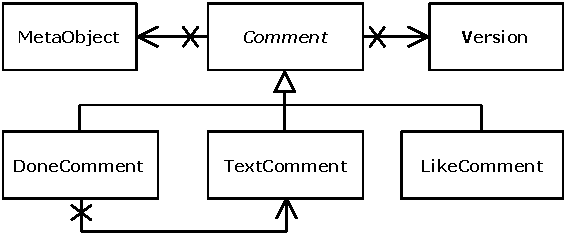
\includegraphics[width=\columnwidth]{images/Overview.pdf}
\caption{Overview over the comment model. Each comment references a meta object (e.g. class, method, package) and references a version encoding the state on which it was commented. A comment can consist of textual feedback or a like action or a done action referencing the comment that should be archived.}
\label{overview}
\end{figure}
\section{Walkthrough}
The developer Alice reads a piece of code relevant to her current issue.
%
She does not understand, why this is done like it is and just adds a comment on this piece of code. 
%
Because Bob did the last change to this code, he gets an email informing him about the new comment. 
%
He opens the concerned method and answers to the questions. 
%
Alice recommends Bob to refactor the code to directly reveal this intention.
%
He does so and pushes the done button of the comment in order to hide the comment of the discussion. 
%
After Alice has finished her issue, Bob enjoys reading her code and therefore pushes the "I like" button of the new method in order to help new developer getting to know the coding styles of the project. 

\section{Main Design Decisions}

\subsection{Client-Server-Architecture}
In order to exchange the comments across the team, a central data storage is needed. 
%
One simple solution would be to attach the comments in custom fields of a commit of the version control software. 
%
But this enforces users to perform a commit after commenting on source code, which is impossible when the developer has no write access to the coded that was commented. 
%
Therefore we implemented this tool using a client-server architecture with. 
%
The server manages the comments in a database and the client created, modifies and shows the comments in the IDE. 
\subsection{Hiding Comments using an explicit Done Button}
Comments that have been discussed and resolved should not be displayed to the developers any more. 
%
Our first intuition was, that a comment should be hidden when the method was changed. 
%
But this leads to problem when the change does not correspond to the comment (e.g. the comment criticizes the name of a method and a developer adds one call inside the method). 
%
Many other scenarios could lead to hiding a comment that is still applicable. 
%
Therefore we decided to keep all comments until they are explicitly marked as done by one developer.  
\begin{comment}
\subsection{Identity of Meta Objects}
In order to connect a comment with a meta object (package, class or method), a reference identifier for these meta objects should be defined. 
%
We chose to reference 
\end{comment}
\section{Related Work}
Many projects working with feature branches perform code reviews during pull requests before merging the changes into the main branch~\cite{driessen2010successful, calefato2015PLE, yu2015pullrequests, tsay2014contributionGithub, gousios2014PullBasedSD, rahman2014pullrequests, tsay2014ContributionDiscussion}. 
%
Tools like CodeFlow~\cite{bird2015CodeReviewPlatform}, Mondrian~\cite{kennedy2006Mondrian}, Gerrit~\cite{google2016gerrit},  Phabricator~\cite{tsotsis2011Phabricator} and ClusterChanges~\cite{barnett2015helpingdevelopers} support these change-based code reviews.
%
In contrast to that, our concept gives feedback on the current state of code instead of a change. 
%
The reviews supported by these tools are made using a push model, meaning that developer request reviews, while our tool uses a pull model, meaning that developers can comment on any code.
%
Hence our concept allows to comment on library code and framework code and therefore give feedback to the developers of third party software. 
%
Furthermore our feedback is continuous and therefore allows new developers to comment on old code. 
%
In contrast to existing tools, our concept allows the developers to stay inside their IDE and avoid context switches. 
%
This provides a more self-sustaining environment that supports the liveness of the development process. 
%
However a dedicated review process before merging changes into the main branch let the developers focus on issues raised up by the specific changes. 
%
Therefore we propose to use our concept in conjunction with pull requests or	 other change-based reviews and not instead of it.
%
\\

%
Discussions and questions about the source code traditionally are done using mailing lists~\cite{vasilescu2014QA}.
%
The recent emergence of Q\&A sites introduces gamification of archiving reputation for answering questions~\cite{vasilescu2014QA}.
%
But like pull requests, they usually are not done inside the IDE but on a separate StackExchange network like StackOverflow.

\section{Discussion}
Our approach encourages continuous conversations about source code regarding quality and correctness. 
%
It simplifies discussions between distant developers in large organizations or open source projects by providing a community platform that forwards a comment automatically to the author of the concerned code.
%
Furthermore, we argue, that using this approach, many source code comment will move out of the code base into the social coding comment database. 
%
This keeps the code clean and focused.
%

%
Our tool minimizes context switching, because code reviews can be done while reading other code without enforcing to switch tasks. 
%
Therefore it integrates well in lean software developement~\cite{poppendieck2003lean} and other agile processes. 
%

%
Unfortunately we did not find any solution how to deal with developers working on the project but not having installed our tool. 
%
This could lead to inconsistent states for examples, when this developer moves a method that is attached by a comment. 
%
Therefore this tool does only work correctly if all working developers have installed our tool. 
\section{Conclusion}
We proposed a tool that helps developers continuously giving feedback on code quality and potential mistakes.
%
This is one contribution for social coding towards a constructive programming society with collective code ownership. 
%
Furthermore it is a contribution for the vision of a self-sustaining IDE by providing a tool for code reviews as one important process for code improvements. 

% An example of a floating figure using the graphicx package.
% Note that \label must occur AFTER (or within) \caption.
% For figures, \caption should occur after the \includegraphics.
% Note that IEEEtran v1.7 and later has special internal code that
% is designed to preserve the operation of \label within \caption
% even when the captionsoff option is in effect. However, because
% of issues like this, it may be the safest practice to put all your
% \label just after \caption rather than within \caption{}.
%
% Reminder: the "draftcls" or "draftclsnofoot", not "draft", class
% option should be used if it is desired that the figures are to be
% displayed while in draft mode.
%
%\begin{figure}[!t]
%\centering
%\includegraphics[width=2.5in]{myfigure}
% where an .eps filename suffix will be assumed under latex, 
% and a .pdf suffix will be assumed for pdflatex; or what has been declared
% via \DeclareGraphicsExtensions.
%\caption{Simulation Results}
%\label{fig_sim}
%\end{figure}

% Note that IEEE typically puts floats only at the top, even when this
% results in a large percentage of a column being occupied by floats.


% An example of a double column floating figure using two subfigures.
% (The subfig.sty package must be loaded for this to work.)
% The subfigure \label commands are set within each subfloat command, the
% \label for the overall figure must come after \caption.
% \hfil must be used as a separator to get equal spacing.
% The subfigure.sty package works much the same way, except \subfigure is
% used instead of \subfloat.
%
%\begin{figure*}[!t]
%\centerline{\subfloat[Case I]\includegraphics[width=2.5in]{subfigcase1}%
%\label{fig_first_case}}
%\hfil
%\subfloat[Case II]{\includegraphics[width=2.5in]{subfigcase2}%
%\label{fig_second_case}}}
%\caption{Simulation results}
%\label{fig_sim}
%\end{figure*}
%
% Note that often IEEE papers with subfigures do not employ subfigure
% captions (using the optional argument to \subfloat), but instead will
% reference/describe all of them (a), (b), etc., within the main caption.


% An example of a floating table. Note that, for IEEE style tables, the 
% \caption command should come BEFORE the table. Table text will default to
% \footnotesize as IEEE normally uses this smaller font for tables.
% The \label must come after \caption as always.
%
%\begin{table}[!t]
%% increase table row spacing, adjust to taste
%\renewcommand{\arraystretch}{1.3}
% if using array.sty, it might be a good idea to tweak the value of
% \extrarowheight as needed to properly center the text within the cells
%\caption{An Example of a Table}
%\label{table_example}
%\centering
%% Some packages, such as MDW tools, offer better commands for making tables
%% than the plain LaTeX2e tabular which is used here.
%\begin{tabular}{|c||c|}
%\hline
%One & Two\\
%\hline
%Three & Four\\
%\hline
%\end{tabular}
%\end{table}


% Note that IEEE does not put floats in the very first column - or typically
% anywhere on the first page for that matter. Also, in-text middle ("here")
% positioning is not used. Most IEEE journals/conferences use top floats
% exclusively. Note that, LaTeX2e, unlike IEEE journals/conferences, places
% footnotes above bottom floats. This can be corrected via the \fnbelowfloat
% command of the stfloats package.

% conference papers do not normally have an appendix


% use section* for acknowledgement

\section*{Acknowledgment}
I would like to thank Patrick Rein for his support and the HPI software architecture group for the continous feedback.
% trigger a \newpage just before the given reference
% number - used to balance the columns on the last page
% adjust value as needed - may need to be readjusted if
% the document is modified later
%\IEEEtriggeratref{8}
% The "triggered" command can be changed if desired:
%\IEEEtriggercmd{\enlargethispage{-5in}}

% references section

% can use a bibliography generated by BibTeX as a .bbl file
% BibTeX documentation can be easily obtained at:
% http://www.ctan.org/tex-archive/biblio/bibtex/contrib/doc/
% The IEEEtran BibTeX style support page is at:
% http://www.michaelshell.org/tex/ieeetran/bibtex/
%\bibliographystyle{IEEEtran}
% argument is your BibTeX string definitions and bibliography database(s)
%\bibliography{IEEEabrv,../bib/paper}
%
% <OR> manually copy in the resultant .bbl file
% set second argument of \begin to the number of references
% (used to reserve space for the reference number labels box)
	
\bibliographystyle{ieeetr}
\bibliography{IEEEabrv,bibliography}


% that's all folks
\end{document}


